% Options for packages loaded elsewhere
\PassOptionsToPackage{unicode}{hyperref}
\PassOptionsToPackage{hyphens}{url}
%
\documentclass[
  9pt,
]{extbook}
\usepackage{lmodern}
\usepackage{amsmath}
\usepackage{ifxetex,ifluatex}
\ifnum 0\ifxetex 1\fi\ifluatex 1\fi=0 % if pdftex
  \usepackage[T1]{fontenc}
  \usepackage[utf8]{inputenc}
  \usepackage{textcomp} % provide euro and other symbols
  \usepackage{amssymb}
\else % if luatex or xetex
  \usepackage{unicode-math}
  \defaultfontfeatures{Scale=MatchLowercase}
  \defaultfontfeatures[\rmfamily]{Ligatures=TeX,Scale=1}
\fi
% Use upquote if available, for straight quotes in verbatim environments
\IfFileExists{upquote.sty}{\usepackage{upquote}}{}
\IfFileExists{microtype.sty}{% use microtype if available
  \usepackage[]{microtype}
  \UseMicrotypeSet[protrusion]{basicmath} % disable protrusion for tt fonts
}{}
\makeatletter
\@ifundefined{KOMAClassName}{% if non-KOMA class
  \IfFileExists{parskip.sty}{%
    \usepackage{parskip}
  }{% else
    \setlength{\parindent}{0pt}
    \setlength{\parskip}{6pt plus 2pt minus 1pt}}
}{% if KOMA class
  \KOMAoptions{parskip=half}}
\makeatother
\usepackage{xcolor}
\IfFileExists{xurl.sty}{\usepackage{xurl}}{} % add URL line breaks if available
\IfFileExists{bookmark.sty}{\usepackage{bookmark}}{\usepackage{hyperref}}
\hypersetup{
  pdftitle={The Live Textbook of Physical Chemistry 2},
  pdfauthor={Dr.~Roberto Peverati},
  hidelinks,
  pdfcreator={LaTeX via pandoc}}
\urlstyle{same} % disable monospaced font for URLs
\usepackage{longtable,booktabs}
\usepackage{calc} % for calculating minipage widths
% Correct order of tables after \paragraph or \subparagraph
\usepackage{etoolbox}
\makeatletter
\patchcmd\longtable{\par}{\if@noskipsec\mbox{}\fi\par}{}{}
\makeatother
% Allow footnotes in longtable head/foot
\IfFileExists{footnotehyper.sty}{\usepackage{footnotehyper}}{\usepackage{footnote}}
\makesavenoteenv{longtable}
\usepackage{graphicx}
\makeatletter
\def\maxwidth{\ifdim\Gin@nat@width>\linewidth\linewidth\else\Gin@nat@width\fi}
\def\maxheight{\ifdim\Gin@nat@height>\textheight\textheight\else\Gin@nat@height\fi}
\makeatother
% Scale images if necessary, so that they will not overflow the page
% margins by default, and it is still possible to overwrite the defaults
% using explicit options in \includegraphics[width, height, ...]{}
\setkeys{Gin}{width=\maxwidth,height=\maxheight,keepaspectratio}
% Set default figure placement to htbp
\makeatletter
\def\fps@figure{htbp}
\makeatother
\setlength{\emergencystretch}{3em} % prevent overfull lines
\providecommand{\tightlist}{%
  \setlength{\itemsep}{0pt}\setlength{\parskip}{0pt}}
\setcounter{secnumdepth}{5}
\usepackage{booktabs}
\usepackage{pdfpages}
\usepackage{amsthm}
\usepackage[version=4]{mhchem}
\usepackage{cancel}

%change to a smaller page:
\usepackage[paperwidth=6in, paperheight=9in]{geometry}
% this is to change the size of text: headsep=10pt, textheight=550pt
%\usepackage[textwidth=456pt]{geometry}

%fancyhdr to set custom headers for the book:
\usepackage{fancyhdr}
\pagestyle{fancy}
\fancyhf{}
\fancyhead[LO]{\slshape\nouppercase{\rightmark}}
\fancyhead[RE]{\slshape\nouppercase{\leftmark}}
\fancyhead[RO,LE]{\thepage}

\makeatletter
\def\thm@space@setup{%
  \thm@preskip=8pt plus 2pt minus 4pt
  \thm@postskip=\thm@preskip
}
\makeatother
\let\oldmaketitle\maketitle
\AtBeginDocument{\let\maketitle\relax}
\ifluatex
  \usepackage{selnolig}  % disable illegal ligatures
\fi
\usepackage[]{natbib}
\bibliographystyle{apalike}

\title{The Live Textbook of Physical Chemistry 2}
\author{\href{mailto:rpeverati@fit.edu}{Dr.~Roberto Peverati}}
\date{04 January 2021}

\begin{document}
\maketitle

%Frontpage for 6x9:
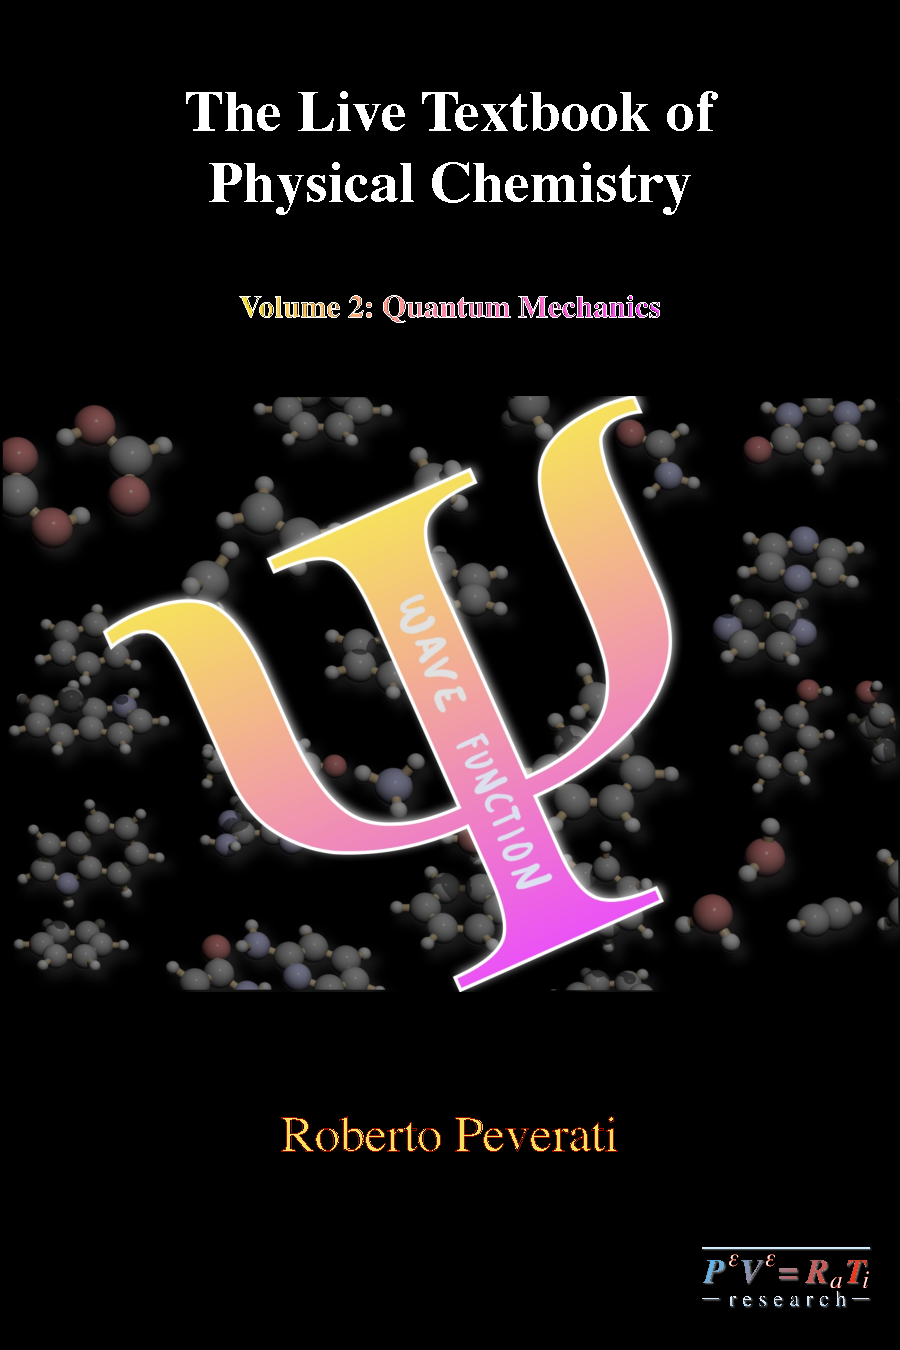
\includepdf[pages={1}, scale=1]{FrontPage_6x9.pdf}
%Frontpage for USLetter:
%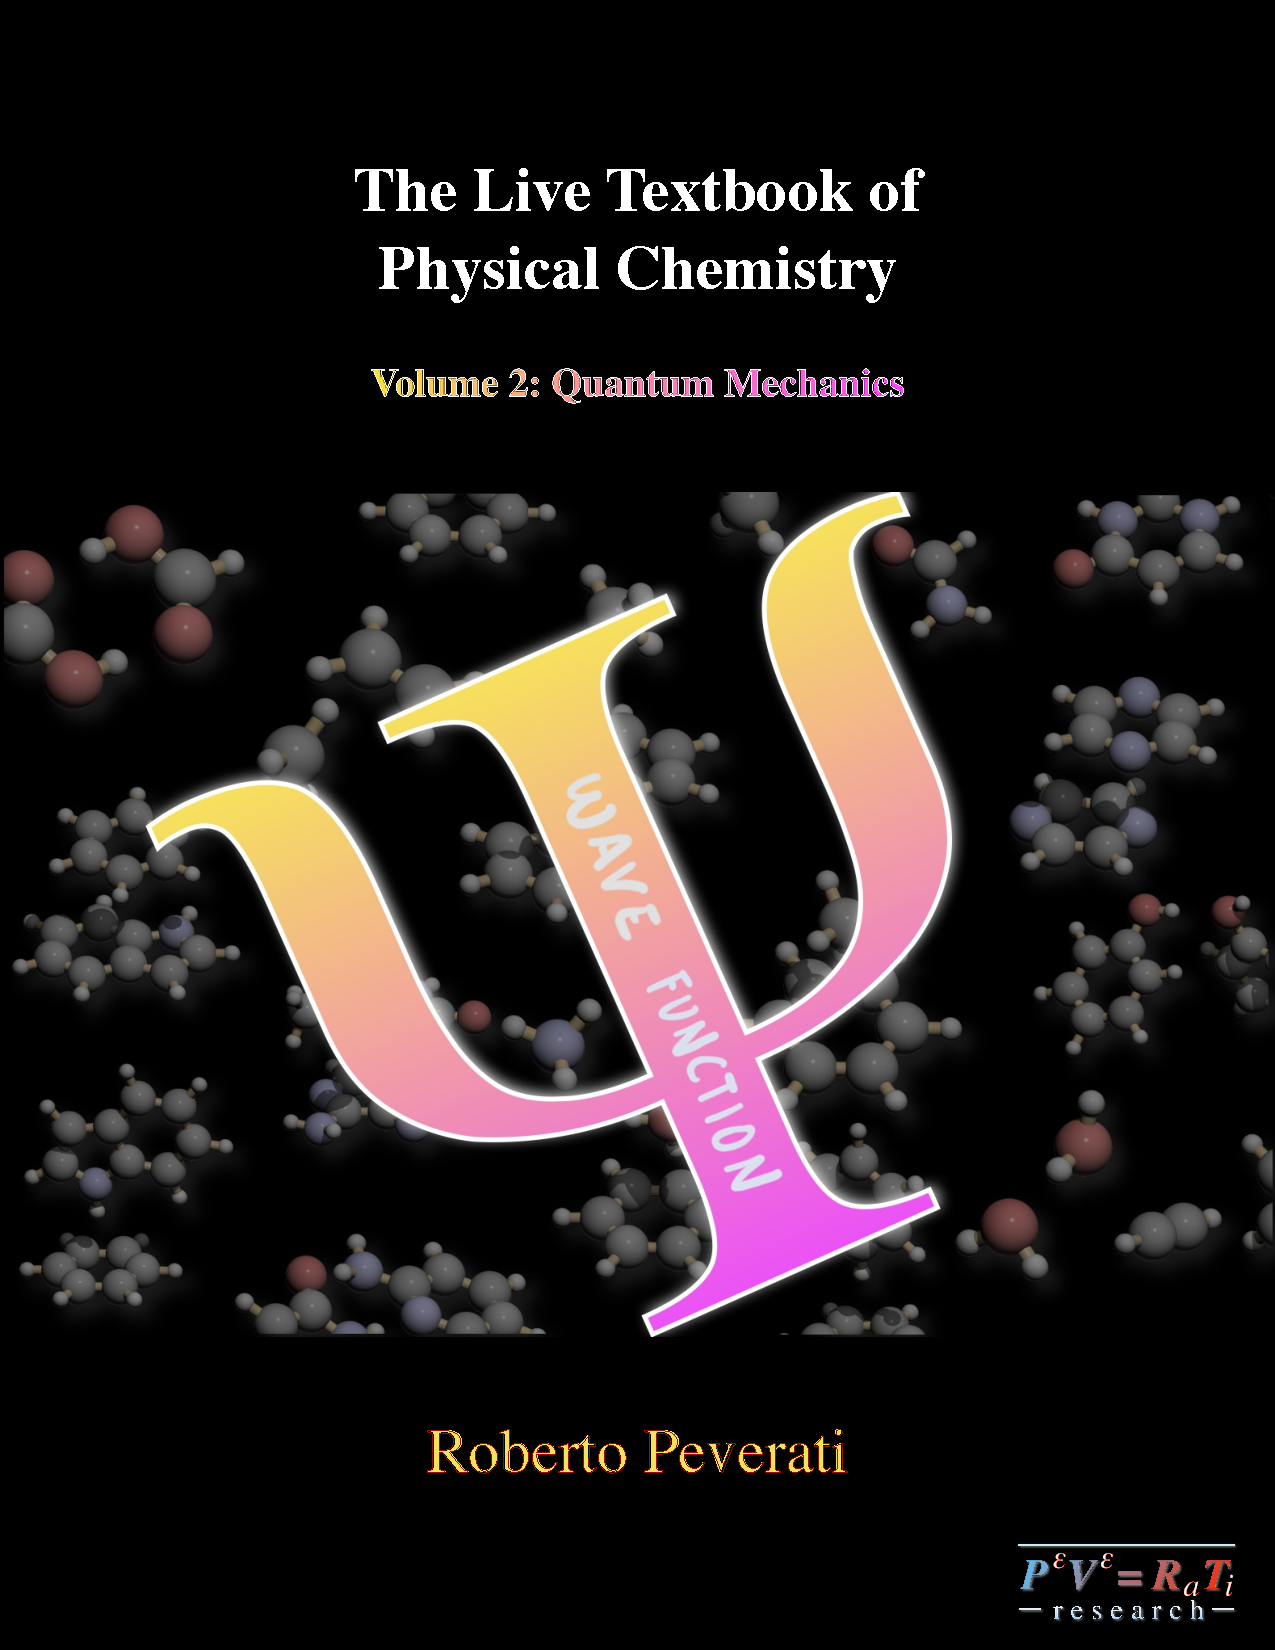
\includepdf[pages={1}, scale=1]{FrontPage.pdf}
\newpage

\let\maketitle\oldmaketitle

% Let's change \thepage so it prints one less than
% the real page number; \pagenumbering{arabic}
% will redefine it to the right meaning afterwards.
\renewcommand\thepage{\romannumeral\numexpr\value{page}-1\relax}


{
\setcounter{tocdepth}{1}
\tableofcontents
}
\renewcommand{\arraystretch}{1.8}

\hypertarget{preface}{%
\chapter*{Preface}\label{preface}}
\addcontentsline{toc}{chapter}{Preface}

\begin{center}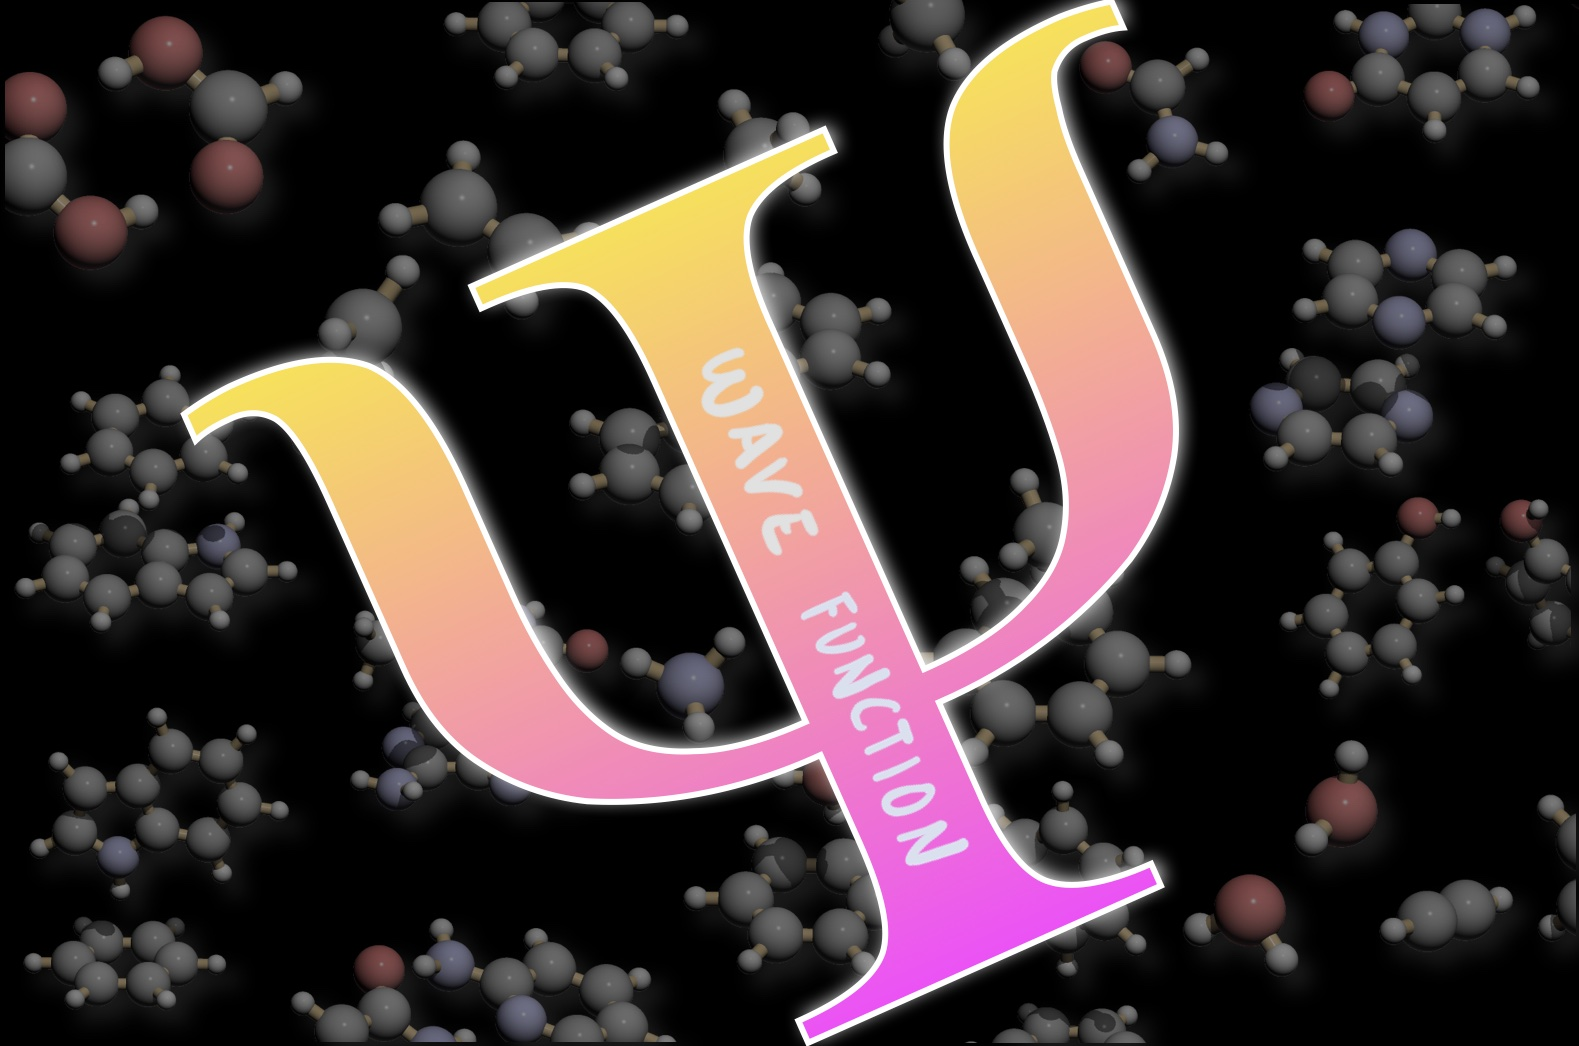
\includegraphics[width=0.8\linewidth]{./img/OEP_Figures.000} \end{center}

This textbook is the official textbook for the Physical Chemistry 2 Course (CHM 3002) at Florida Tech.

The instructor for this course and author of this textbook is Dr.~Roberto Peverati.

\textbf{Contacts}: \href{mailto:rpeverati@fit.edu}{\nolinkurl{rpeverati@fit.edu}}, Office: OPS 333, (321) 674-7735

Chemistry Program, Department of Biomedical and Chemical Engineering and Science
Florida Institute of Technology, Melbourne, FL.

\begin{quote}
This live open textbook is distributed under the \href{https://creativecommons.org/licenses/by-sa/4.0/}{CC-BY-SA 4.0 License} and it was funded by the Florida Tech Open Educational Resources Grant Program: A Collaboration of the Teaching Council, eEducation, and the Evans Library.
\end{quote}

\hypertarget{how-to-use-this-book}{%
\section*{How to use this book}\label{how-to-use-this-book}}
\addcontentsline{toc}{section}{How to use this book}

If you have taken P-Chem 1 at Florida Tech in the Fall Semester 2020, you should already be familiar with this format. Everything we did with the Live Textbook of P-Chem 1 in FS2020 will be happening this semester with P-Chem 2. Please read this book carefully, since everything that will be in your exams is explained here.
Since this book is specifically tailored for the CHM 3002 course at Florida Tech, there are no superfluous parts. In other words, everything in it might be subject to question in the quizzes and the final exam.

\begin{quote}
Definitions and exercises are usually numbered and are highlighted in the text in this format (lighter grey, indented, and following a grey vertical bar). Please study the definitions carefully since they are fundamental concepts that will be used several times in the remainder of the text, and they will be subject to quizzes and exams. Exercises are essential for cementing the concepts, and you should attempt to execute them first without looking at the solution. Even if you were able to solve an exercise on your own, always read the solution after, since it might contain additional explanations expanding the main concepts in the text.
\end{quote}

Navigating the book should be straightforward. On each page, there is a useful sidebar on the left that gives you an overview of all chapters, and a toolbar at the top with important tools. Arrows to shift between chapters might also be present, depending on your browser. If you are old-school and prefer a pdf, you can download a printout by clicking on the toolbar's corresponding icon. If you are \emph{really} old-school and prefer a printed book, the best solution is to download the pdf and print it yourself. It is a LaTeX book, and I can promise you it will look good on paper. However, I cannot provide physical copies to each student. In the toolbar, you will find a useful search box that is capable of searching the entire book. The most adventurous will find in the toolbar a link to the raw GitHub source code. Feel free to head on \href{https://github.com/peverati/PChem2}{over there} and fork the book.

Each chapter of this book represents one week of work in the classroom and at home. The sidebar on the left will reflect your syllabus, as well as the main structure of the class on Canvas. The book is a live document, which means it will be updated throughout the semester with new material. While you are not required to check it every day, you might want to review each week's chapter before the lecture on Friday.

\begin{quote}
If you spot a mistake or a typo, contact Dr.~Peverati via \href{mailto:rpeverati@fit.edu}{email} and you will receive a credit of up to three points towards your final score, once the typo has been verified and corrected.
\end{quote}

\cleardoublepage
\pagenumbering{arabic}

\hypertarget{Motivation}{%
\chapter{The Motivation for Quantum Mechanics}\label{Motivation}}

\hypertarget{introduction}{%
\section{Introduction}\label{introduction}}

Quantum mechanics is an important intellectual achievement of the 20th century. It is one of the more sophisticated field in physics that has affected our understanding of nano-meter length scale systems important for chemistry, materials, optics, and electronics. The existence of orbitals and energy levels in atoms can only be explained by quantum mechanics. Quantum mechanics can explain the behaviors of insulators, conductors, semi-conductors, and giant magneto-resistance. It can explain the quantization of light and its particle nature in addition to its wave nature. Quantum mechanics can also explain the radiation of hot body, and its change of color with respect to temperature. It explains the presence of holes and the transport of holes and electrons in electronic devices.
Quantum mechanics has played an important role in photonics, quantum electronics, and micro-electronics. But many more emerging technologies require the understanding of quantum mechanics; and hence, it is important that scientists and engineers understand quantum mechanics better. One area is nano-technologies due to the recent advent of nano-fabrication techniques. Consequently, nano-meter size systems are more common place. In electronics, as transistor devices become smaller, how the electrons move through the device is quite different from when the devices are bigger: nano-electronic transport is quite different from micro-electronic transport.
The quantization of electromagnetic field is important in the area of nano-optics and quantum optics. It explains how photons interact with atomic systems or materials. It also allows the use of electromagnetic or optical field to carry quantum information. Moreover, quantum mechanics is also needed to understand the interaction of photons with materials in solar cells, as well as many topics in material science.
When two objects are placed close together, they experience a force called the Casimir force that can only be explained by quantum mechanics. This is important for the understanding of micro/nano-electromechanical sensor systems (M/NEMS). Moreover, the understanding of spins is important in spintronics, another emerging technology where giant magneto-resistance, tunneling magneto-resistance, and spin transfer torque are being used.
Quantum mechanics is also giving rise to the areas of quantum information, quantum 1
2 Quantum Mechanics Made Simple communication, quantum cryptography, and quantum computing. It is seen that the richness
of quantum physics will greatly affect the future generation technologies in many aspects.

\hypertarget{quantum-mechanics-is-bizarre}{%
\section{Quantum Mechanics is Bizarre}\label{quantum-mechanics-is-bizarre}}

The development of quantum mechanicsis a great intellectual achievement, but at the same time, it is bizarre. The reason is that quantum mechanics is quite different from classical physics. The development of quantum mechanics is likened to watching two players having a game of chess, but the watchers have not a clue as to what the rules of the game are. By observations, and conjectures, finally the rules of the game are outlined. Often, equations are conjectured like conjurors pulling tricks out of a hat to match experimental observations. It is the interpretations of these equations that can be quite bizarre.
Quantum mechanics equations were postulated to explain experimental observations, but the deeper meanings of the equations often confused even the most gifted. Even though Einstein received the Nobel prize for his work on the photo-electric effect that confirmed that light energy is quantized, he himself was not totally at ease with the development of quantum mechanicsas charted by the younger physicists. He was never comfortable with the probabilistic interpretation of quantum mechanics by Born and the Heisenberg uncertainty principle: ``God doesn't play dice,'' was his statement assailing the probabilistic interpretation. He proposed ``hidden variables'' to explain the random nature of many experimental observations. He was thought of as the ``old fool'' by the younger physicists during his time.
Schrödinger came up with the bizarre ``Schrödinger cat paradox'' that showed the struggle that physicists had with quantum mechanics's interpretation. But with today's understanding of quantum mechanics, the paradox is a thing of yesteryear.
The latest twist to the interpretation in quantum mechanics is the parallel universe view that explains the multitude of outcomes of the prediction of quantum mechanics. All outcomes are possible, but with each outcome occurring in different universes that exist in parallel with respect to each other.\footnote{This section was adapted in part from Prof.~Weng Cho CHEW's Quantum Mechanics Made Simple Lecture Notes available \href{http://wcchew.ece.illinois.edu/chew/course/qmall20121005.pdf}{here}.}

The development of quantum mechanics was initially motivated by two observations which demonstrated the inadeqacy of classical physics. These are the ``ultraviolet catastrophe'' and the photoelectric effect.

\hypertarget{the-ultraviolet-catastrophe}{%
\section{The Ultraviolet Catastrophe}\label{the-ultraviolet-catastrophe}}

A blackbody is an idealized object which absorbs and emits all frequencies. Classical physics can be used to derive an equation which describes the intensity of blackbody radiation as a function of frequency for a fixed temperature--the result is known as the Rayleigh-Jeans law. Although the Rayleigh-Jeans law works for low frequencies, it diverges as \(\nu^2\); this divergence for high frequencies is called the ultraviolet catastrophe.
Max Planck explained the blackbody radiation in 1900 by assuming that the energies of the oscillations of electrons which gave rise to the radiation must be proportional to integral multiples of the frequency, i.e.,

\begin{equation}
E = n h \nu
\label{eq:uvcat}
\end{equation}

Using statistical mechanics, Planck derived an equation similar to the Rayleigh-Jeans equation, but with the adjustable parameter \(h\). Planck found that for \(h = 6.626 \times 10^{-34}\) J s, the experimental data could be reproduced. Nevertheless, Planck could not offer a good justification for his assumption of energy quantization. Physicicsts did not take this energy quantization idea seriously until Einstein invoked a similar assumption to explain the photoelectric effect.

\hypertarget{the-photoelectric-effect}{%
\section{The Photoelectric Effect}\label{the-photoelectric-effect}}

In 1886 and 1887, Heinrich Hertz discovered that ultraviolet light can cause electrons to be ejected from a metal surface. According to the classical wave theory of light, the intensity of the light determines the amplitude of the wave, and so a greater light intensity should cause the electrons on the metal to oscillate more violently and to be ejected with a greater kinetic energy. In contrast, the experiment showed that the kinetic energy of the ejected electrons depends on the frequency of the light. The light intensity affects only the number of ejected electrons and not their kinetic energies.
Einstein tackled the problem of the photoelectric effect in 1905. Instead of assuming that the electronic oscillators had energies given by Planck's formula, eq. \eqref{eq:uvcat}, Einstein assumed that the radiation itself consisted of packets of energy \(E = h \nu\), which are now called photons. Einstein successfully explained the photoelectric effect using this assumption, and he calculated a value of \(h\) close to that obtained by Planck.

Two years later, Einstein showed that not only is light quantized, but so are atomic vibrations. Classical physics predicts that the molar heat capacity at constant volume (\(C_v\)) of a crystal is \(3 R\), where \(R\) is the molar gas constant. This works well for high temperatures, but for low temperatures \(C_v\) actually falls to zero. Einstein was able to explain this result by assuming that the oscillations of atoms about their equilibrium positions are quantized according to \(E = n h \nu\), Planck's quantization condition for electronic oscillators. This demonstrated that the energy quantization concept was important even for a system of atoms in a crystal, which should be well-modeled by a system of masses and springs (i.e., by classical mechanics).\footnote{The previous 2 sections were adapted in part from Prof.~C. David Sherrill's A Brief Review of Elementary Quantum Chemistry Notes available \href{A\%20Brief\%20Review\%20of\%20Elementary\%20Quantum\%20Chemistry}{here}.}

\hypertarget{Classical}{%
\chapter{Classical Mechanics and Wave Mechanics}\label{Classical}}

\end{document}
